
\documentclass[a4paper]{article}
 
% A simple Latex document illustrating some of the main document features

\usepackage{natbib}
\usepackage{float}
\usepackage{setspace}
\usepackage{textcmds}
\usepackage{graphicx}
\usepackage{changepage}
\usepackage[section]{placeins}

\begin{document}

\title{Data Mining the Healthcare Dataset: Report}
\author{100227404}
\date{} % Leave this empty if you prefere
\maketitle

\section{Abstract}
This project explores a medical dataset used to asses risk related to a particular unknown condition. The data is explored and visualised, then sever preprocessing methods are proposed before, supervised and unsupervised learning methods are used to attempt to label the data.

\section{Data exploration, visualisation, and summary} \label{intro}

\subsection*{Introduction to the dataset}

This is a dataset of medical data. In total there are 4250 records in the dataset and a possible 24 variables recorded per record, of which one if an identifier and one is a target variable. The target variable is broken into three levels low\_risk, moderate\_risk nd high\_risk. Of all 24 variables, 22 are available to potentially be used as predictors. 

\subsection*{Variable types}

All 24 of the variables are one of four distinct variable types. They are boolean, true categorical, integers and rationals. The variables are listed and divided by type below;

\begin{itemize}
    \item \textbf{Boolean:} sick, pregnant, concern\_type1, concern\_type2,
                           enlargement, tumor, disorder, medication\_A,
                           medication\_B, mental\_health, mood\_stabiliser, surgery,
                           treatment\_type1, suspect
    \item \textbf{Categorical:} id, gender, target
    \item \textbf{Integer:} age
    \item \textbf{Rational:} test\_X1, test\_X2, test\_X3, test\_X4, test\_X5, test\_X6
\end{itemize}

\noindent These are combined into two groups those being Numerical and categorical.

\begin{itemize}
    \item \textbf{Categorical:} sick, pregnant, concern\_type1, concern\_type2,
                           enlargement, tumor, disorder, medication\_A,
                           medication\_B, mental\_health, mood\_stabiliser, surgery,
                           treatment\_type1, suspect, id, gender, target
    \item \textbf{Numerical:} age, test\_X1, test\_X2, test\_X3, test\_X4, test\_X5, test\_X6
\end{itemize}

\subsection*{Missing values and outliers}

Identifying the number of missing values in each variable measurement is important when deciding whether or not variables can be used, as such the missing values from each variable are counted. The number of missing values and the percentage of records they occupy is listed below in descending order.
test\_X6   4096 (96.4\%), test\_X2   1243 (29.2\%), test\_X1   411 (9.67\%), test\_X4   392 (9.22\%), test\_X5   387 (9.11\%), test\_X3   216 (5.01\%), gender   141 (3.32\%).
% \begin{enumerate}
%     \item test\_X6   4096 (96.4\%)
%     \item test\_X2   1243 (29.2\%)
%     \item test\_X1   411 (9.67\%)
%     \item test\_X4   392 (9.22\%)
%     \item test\_X5   387 (9.11\%)
%     \item test\_X3   216 (5.01\%)
%     \item gender   141 (3.32\%)
% \end{enumerate}

These percentages and values become relevant in pre-processing. Identifying outliers is equally as important as identifying missing values. For age as a variable this is reasonably easy since it's incredibly unlikely there's anyone in the data over 100 years old, and impossible anyone over 120 years old is in the data, likewise it's impossible for anyone to have a negative age. So specifying these conditions we see if there exist any records outside these ranges, two such records exist ages 65526 and 455. These records are immediately removed from the dataset (their removal is further explained in section \ref{removal}).

Unfortunately from the data it's impossible to identify what tests one through six are actually testing for and how, hence it's hard to identify outliers from mere inspection. It's even more difficult to identify outliers in categorical data. We leave this identification to the preprocessing stage. 

\subsection*{Unique values} %CUT IF NECESSARY

To give an indication of the variability of each variable the number on unique values in each column is counted. As would be expected all the boolean variables have two unique values, except disorder which has one. The numerical variables all have a reasonable number of unique values, as would be expected the number of unique values appears to be related to the number of null-values. Below a graph of the numerical variable to illustrate this;

\begin{figure}[h]
    \centering
    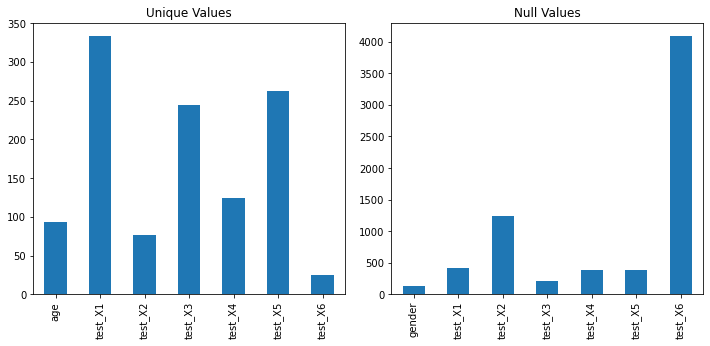
\includegraphics[width=0.75\linewidth]{Materials/Barplots/Unique_Null.png}
    \caption{A comparison of null and unique values for numerical variables}
    \label{fig:Unique_Null}
    
\end{figure}

On the note of unique values no duplicate rows were found throughout the dataset.

\subsection{Visualisation}

Now to properly explore the variability of the variables several graphs are created, below some of the notable graphs are displayed and explained. (we exclude test 6, the reason for this being in section \ref{removal})

\begin{figure}[ht]
\begin{minipage}[b]{0.45\linewidth}
\centering
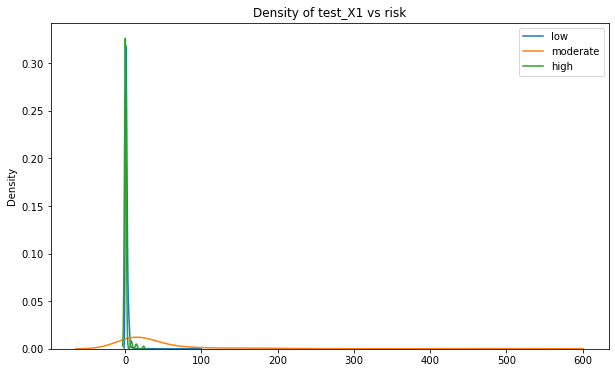
\includegraphics[width=\textwidth]{Materials//Density Plots/test1.png}
\end{minipage}
\hspace{0.25cm}
\begin{minipage}[b]{0.45\linewidth}
\centering
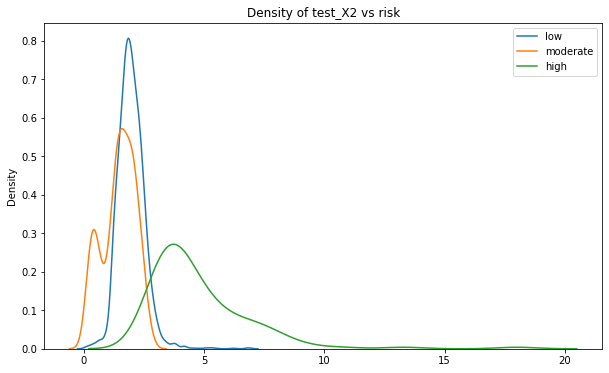
\includegraphics[width=\textwidth]{Materials//Density Plots/test2.png}
\end{minipage}
\caption{Results density of tests 1,2 by target variable}
\label{fig: Density results tests 1,2}
\end{figure}

\begin{figure}[h]
\begin{minipage}[b]{0.45\linewidth}
\centering
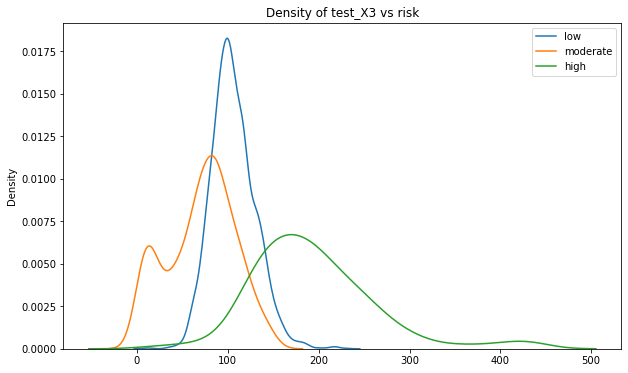
\includegraphics[width=\textwidth]{Materials//Density Plots/test3.png}
\end{minipage}
\hspace{0.25cm}
\begin{minipage}[b]{0.45\linewidth}
\centering
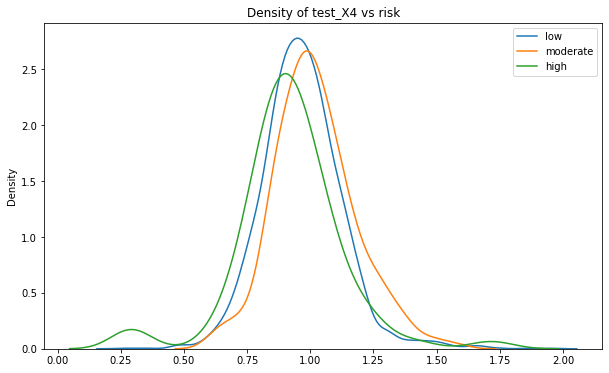
\includegraphics[width=\textwidth]{Materials//Density Plots/test4.png}
\end{minipage}
\caption{Results density of tests 3,4 by target variable}
\label{fig: Density results tests 3,4}
\end{figure}

\begin{figure}[h]
\begin{minipage}[b]{0.45\linewidth}
\centering
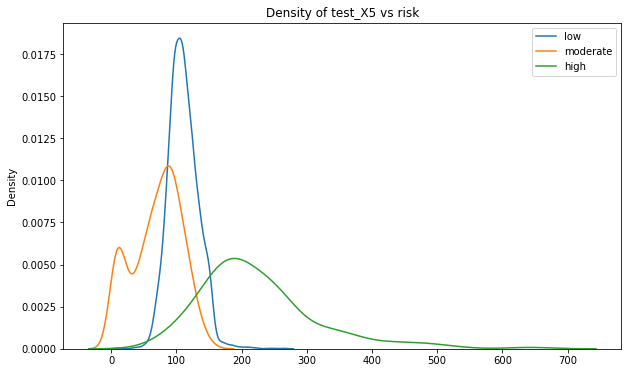
\includegraphics[width=\textwidth]{Materials//Density Plots/test5.png}
\end{minipage}
\hspace{0.25cm}
\begin{minipage}[b]{0.45\linewidth}
\centering
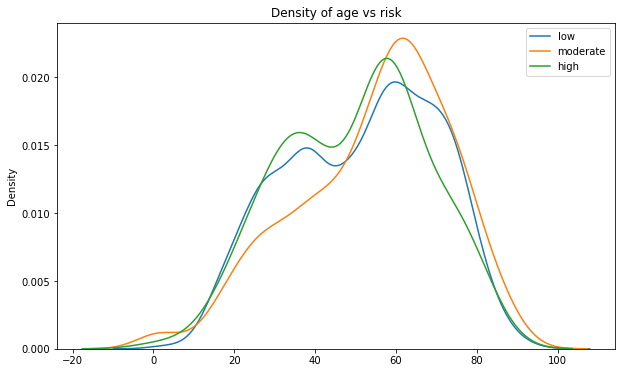
\includegraphics[width=\textwidth]{Materials//Density Plots/Age.png}
\end{minipage}
\caption{Results density of test 5 and age  by target variable}
\label{fig: Density results test 5 and age}
\end{figure}

As seen in figures \ref{fig: Density results tests 3,4} and \ref{fig: Density results test 5 and age}, tests 3 and 5 seem to have similar distributions and axis. This could indicate overlap in the information contained in these tests. 

Tests 2,3,5 share distributions while not necessarily axis. Most notably with moderate risk appearing to be bimodal. An interpretation of this could mean that all three tests are looking at a similar medical indicator even if they might test for it in different ways. To compare we plot a pairwise scatter plot of these tests, and return to this question of how related they are in section \ref{tests}

\begin{figure}[h]
    \centering
    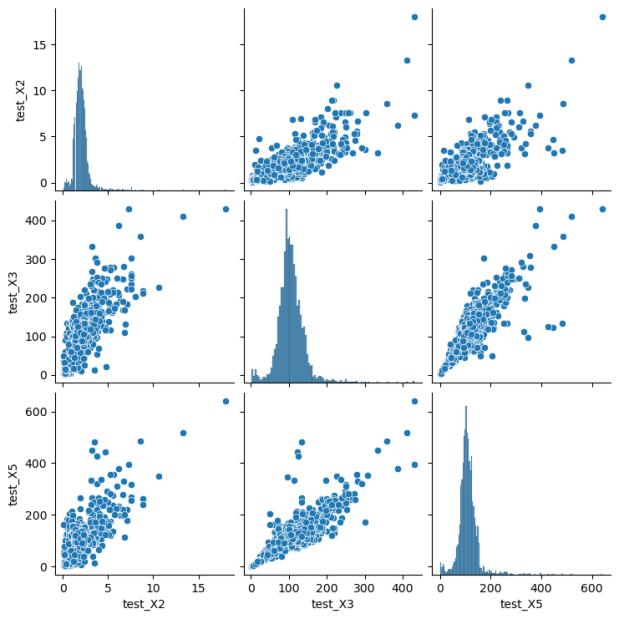
\includegraphics[width=0.75\linewidth]{scatter_pair_2_3_5.png}
    \caption{Scatter plot of tests 2,3 and 5 compared}
    \label{fig:235 scatter}
\end{figure}

Interestingly in almost the opposite moderate risk is far closer to being mono-modal with low and high risk being bimodal for age. with the risk generally increasing with age past 10 and again at around 45.

Tests 1 and 4 don't seem to share their distributions with any of the other tests, and both have a considerable amount of overlap between risk groups likely indicating they contain less information that can be used to distinguish target variables. Despite this test 4 might have a trimodal distribution for high risk which makes it useful, similarly test 1 has a lot more variance for moderate risk which again makes it useful.

The categorical variables are plotted as box plots separated out by risk. From every graph of a boolean variable there's an indication that the majority of the respondents answered no, this is not exceptional for medical data but does mean a considerable number of these measurements are unlikely to be good predictors. 
For example; 
of all the records only 62 had surgery filled out as yes and of them only 3 of them outside of the low\_risk target variable. It's also worth asking with variables like surgery and tumor if survival bias might be a contributing factor, we don't know how the data was gathered so it's difficult to tell but it is a possibility. 

Despite this there are some categorical variables that may contain information, as an example the graphs for medication A (figure \ref{fig:MedA box}) and gender (figure \ref{fig:gender box}). Medication A has a considerable number of yes responses that are low\_risk, this could mean that medication A has a suppressive effect on the condition we're testing for. And for gender male seems to have less associated risk than female or not\_specified.

\begin{figure}[h]
    \centering
    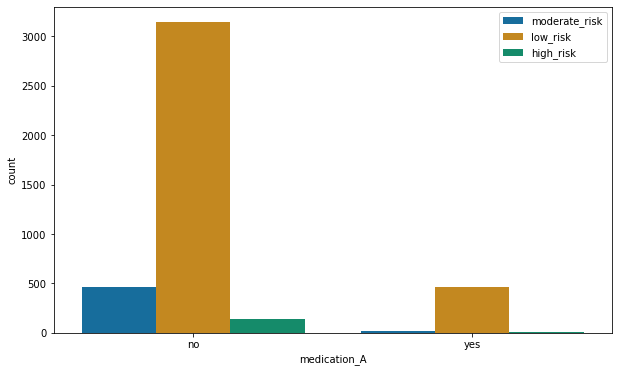
\includegraphics[width=0.75\linewidth]{Materials/Barplots/MedicationA.png}
    \caption{Risk and response bar-plots for Medication A}
    \label{fig:MedA box}
\end{figure}
\begin{figure}[h]
        \centering
        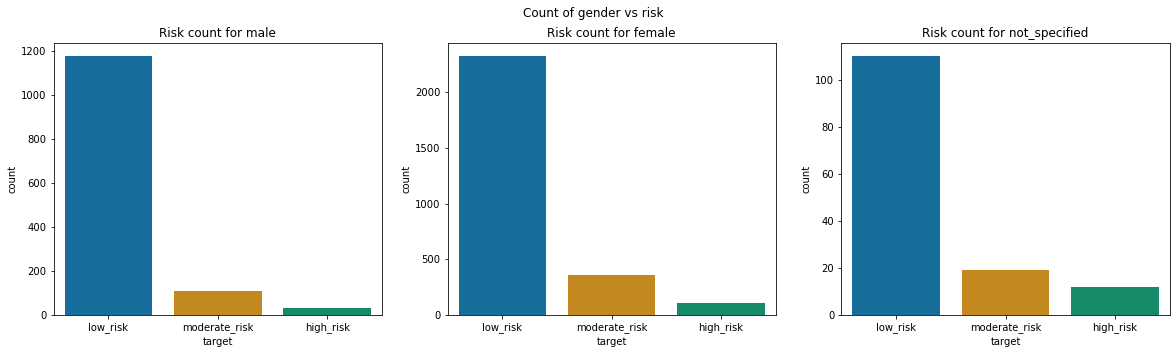
\includegraphics[width=1\linewidth]{Materials/Barplots/Gender.png}
        \caption{Risk box plots by gender}
        \label{fig:gender box}
    \end{figure}

\section{Data Cleansing and preprocessing}

Before data can be handed to any algorithm you need to clean the data and process the data. This involves several steps including; cleansing (null removal/imputation), encoding, outlier detection/removal, balancing, standardisation, train-test-validation splits, feature selection/dimensionality reduction.

The methods are discussed below, for many their usage is saved for the discussion of pipelines.

\subsection{Initial cleansing}\label{removal}

As mentioned previously there are two records with Ages very far outside the reasonable limit, and these records were removed prior to visualisation. Whilst it might be possible to impute Age data there are several reasons that is inadvisable in this case, we have only two records, both records belong to the low risk group which is our majority target class, these records are so far outside reasonable limits for age data it might not be advisable to trust any of the measurements in the record.  

Also mentioned above is that the column disorder has only one value, this makes it entirely useless for the purposes of prediction. Similarly because test 6 has 96.4\% of it's values missing we cannot use this for the purposes of prediction (Hence why it was not graphed). There were no duplicate rows so we don't need to consider removing them


\subsection{Preprocessing Ordering}

Outside of these cleansing steps the remaining steps can be performed in different orders dependant on methods used and the algorithm the data is being fed into. As such the creation of different pipelines to process and save the data or immediately pass the data to algorithms have been explored and implemented.
As such the steps presented and their explanations might not always follow each other or be compatible.

\subsection{Null-handling}
In general sklearn model (which are what is used) aren't robust to null values, and dependant on algorithm being robust to null values can often meaning omitting them or imputing them within a model, as such it makes sense to have several null-handling strategies as an independent step.
Five different methods of null-handling were explored and three of these were implemented. Before any of these methods we want to handle the null values in gender since this is the same for all techniques, for the gender null values we replace them with not\_specified or 'empty'. The reasons are, these values may remain missing from real world data to which we wish to apply our predictions, imputing gender based data can enhance biases that might already be present in the data, we may loose information since not providing gender data might be medically indicative i.e. the data is missing not at random MNAR.

\textbf{Method 1:} Null removal, This is the simplest of all the methods and just involves disregarding any row with null information in it. Whilst this method can avoid altering the distribution of the data in our particular case it can limit the possible feature selection depending on how much data we are okay with disregarding 

\textbf{Method 2:} Mean Imputation, To do this you replace all missing values in a column with the mean value of that column. The problem with this method is that mean as a measurement is heavily affected by outliers, hence mean imputation is heavily affected by outliers. Essentially requiring outlier detection and removal before implementation. This method wasn't used since with medical data outlier removal without domain knowledge can cause useful information to be disregarded.

\textbf{Method 3:} Median Imputation, As with mean imputation you replace all of a columns values with the median value from that column. Unlike mean imputation this isn't as affected by outliers, however with the data we have we risk altering the distribution of the data especially with any data that is multi-modal. Thankfully without regard to target classes our data is mostly mono-modal. 

\textbf{Method 4:} Knn Imputation, This method is more powerful than the previous two since it doesn't assume any underlying distribution in the data. It works like a K-nearest Neighbour (knn) classifier by using the a number of nearest neighbours to fill the values for an empty cell. The downside of this method is that knn can be inaccurate for variables with different scale lengths, so you should standardise data before performing this method. However standardisation requires outliers be removed. 

\textbf{Method 5:} Multiple imputation, This method uses one method of imputation multiple times to create several different imputed datasets, then analysis is performed on these data sets to create sampling conditions, these conditions let you sample the imputed datasets for imputed values to create a final imputed dataset. In particular Knn imputation with sequential imputation from \cite{faisal2021multiple} was looked at. Whilst this method is promising it's too time consuming and computationally intensive for this project, this method also suffers all the drawbacks of whichever method of imputation is used to create the multiple imputed datasets. 

To summarise, null removal, median imputation and knn imputation are all performed on the dataset dependant on the algorithm used. In theory the choice of imputation strategy can become a hyper-parameter for any algorithm. Methods exist for imputing categorical variables, however it doesn't appear there are any missing values in the categorical data in this dataset as such these methods are not explored.

\subsection{outlier detection/removal}

As expressed above outliers can not only affect the results of an algorithm but the other preprocessing steps themselves, as such identifying and removing outliers can be an essential step in preprocessing. In this report several methods of outlier removal are examined and some of them are implemented. 

\textbf{method:} DB-scan, this method uses clustering to identify outliers, by creating a number of clusters, points at the centre of or inside clusters aren't considered outliers, ones outside clusters are. The size of the clusters and minimum number of points per cluster are parameters that can effect this algorithm, to ensure it was used properly the algorithm was test with a silhouette score and Davies-Boulin index, silhouette score is calculated for every point and measures how well it belongs to it's cluster, so it's similar to cluster separability. Meanwhile Davies-Boulin is a measure of the similarity between clusters. Using both of these the clusters from DB-scan should be well separated and reasonably similar.

\textbf{caveat:} The parameters for DB-Scan used were decided in data exploration, however too late into this project the realization that the data should be scaled before DB-scan is used was realised, this means that the results from DB-scan may not be reflective of real outliers it also means the large epsilon value originally chosen was made smaller

\textbf{method:} Local outlier factor, this method also uses clustering it takes any point calculates it's distance from it's neighbours and compares that to this number for those neighbours. If it has a higher distance than it's neighbours it's more likely to be an outlier.

\textbf{method:} Isolation forest, this method uses a forest which is a collection of decision trees. Each tree randomly splits the data based on a particular feature. The number of splits that isolate a point is considered a measure of how much of an outlier it is.

\subsection{Standardisation}
Several of the methods examined required standardisation beforehand, this is because many of them rely on the distances between multiple measurements, when this is the case non-standardised data can be incorrectly represented, this is due to the preferencing of or against variables with significantly smaller or larger scales than average. As such it's imperative that our scales are standardised to avoid these errors. Both normalisation and standardisation are covered, only standardisation was implemented because of the assumptions of normalisation.

\textbf{method:} Normalising, Standard normalisation involves trying to move all the values onto a standard normal distribution. This is done by taking any value subtracting the mean and dividing by the the standard deviation. There are two problems with this method, it is sensitive to outliers and it assumes that the data is normally distributed. Below an equation for this method is given, where X is a point mu is mean and sigma is a standard deviation.

$$\frac{X-\mu}{\sigma}$$

\textbf{method:} Standardising, This is referring to min-max scaling this places all the values between 0 and 1, it does so by taking any value subtracting the minimum value and dividing by the difference between the minimum and maximum value. As with previous an equation is given below. 

$$\frac{X - X_{min}}{X_{max} - X_{min}}$$

\subsection{Train/Test/Validation split}

The train, test, validation split is a partitioning of the data into three or more sets. Most commonly the training set, validation set and test set. Each one serves a different purpose. Training sets are used to train models, validation sets are used during training to evaluate model performance adjust parameters and more sophisticated processes like automatic stopping, Testing sets are used after a good model is picked to evaluate the data on a set as of yet unseen by the model.

The idea of these partitions is to avoid data leakage, which is when data from one of the partitions affects another in model creation. This is a problem since it can lead to a misrepresentation of accuracy, and hence the best model might not be picked. With all the steps mentioned above there's a danger of data leakage. As such it's generally advisable to perform the train/test/split as early as possible. Train-test split is generally used to partition the data into 80\% training data, 20\% testing data, this is the case for this project.

\textbf{caveat:} There are cases where more partitions are used. For example one can use K-fold cross validation, with this the dataset is divided into K many folds, then each fold is used a validation set once while the model is trained on the remainder of the data. Followed by model evaluation on training data. 

\textbf{caveat:} Stratification refers to drawing from each of the target classes equal, we will use this since it should prevent data in the validation or test set from not being reflective of real world data.  

\subsection{Balancing}

Balancing is a technique used to make a model more generalisable, this is done by making the number of records for each target class equal. This should avoid the model preferencing predicting for any particular class. There are two ways to balance the number of classes, up-sampling and down-sampling. There are various methods for these explored below, some of which are implemented.

\textbf{method:} down-sampling, means taking the majority class and choosing fewer records from it than it contains to reduce it's size.

\textbf{method:} up-sampling (random oversampling), the simplest method of up-sampling is random over sampling which is just picking records and duplicating them, this method can cause over fitting since it directly replicates records. Similarly it can cause issues by replicating outliers.

\textbf{method:} up-sampling (SMOTE), referring to Synthetic Minority Oversampling Technique, is a method of creating samples based on distance so samples are generated near other minority points. As with the previous up-sampling method this method can cause over fitting, it could also falsely inflate the presence of outliers, however since generally it operates on bisecting the line between two other minority class instances it is less prone to this.\textit{From this point onward the usages of these methods are explained as they are described.}

\textbf{particulars:} For this project, a mixture of down-sampling and smote was employed, because of the severe imbalance in the data set. The majority class was down-sampled to 1000 samples, and the two minority classes were up-sampled to 1000 samples each with SMOTE.

\subsection{encoding}
Encoding is a necessary step, it converts data into something that can be used by various algorithms (i.e. turning true, false int 1, 0). Two encoding methods were used. They are explained below.

\textbf{method:} One Hot Encoding, this is a type of encoding whereby the categories of a column become their own columns that are zero for every row except those where that category occurs in the original column.

\textbf{method:} Ordinal-encoding, when there's a natural order to categories ordinal encoding maps that order onto the categories.

\textbf{outcome:} For the data-set the boolean variables were encoded as zero for false, one for true. The target variable was ordinal encoded, with one being low risk, two moderate, risk and three high risk. Gender was one hot encoded, with G\_female, G\_male, G\_empty being the new columns.

\subsection{feature selection} \label{tests}
Feature selection is another name for dimensionality reduction. This means reducing the feature set used to create a model, the idea being that removing features that contribute little to no information shouldn't effect the accuracy of the model, but reducing the dimensionality should improve the accuracy and explain-ability of the model. There are various ways of choosing the key features to maintain, some of them are explored of those some are implemented.

From a small amount of domain knowledge it appears that the test variables are the most likely to be good predictors, while the categorical variables are likely included for completeness, despite this we will perform feature comparison between all variables since some of the categorical appear to contain information relevant to the model (i.e. gender, medication A). In general the methods used can be split into two frameworks, filter methods and wrapper methods. In short filter methods are statistical test applied to data to rank data, wrapper methods are methods that create models with different features sets and through comparing their outcomes choose feature sets that work best.

\textbf{method:} Paired t-test, this is a way of comparing the means of two continuous variables which are drawn from the measuring the same thing. 

\textbf{outcome:} It was used to compare the means of tests 2,3,5 to make sure they're reasonably different from each other (since the results of each record are drawn from one individual this is a pared t-test not independent). Since t-tests are susceptible to outliers, the least significant difference between tests 3,5 is checked with trimmed means (the idea of this being to remove outliers). From these tests the conclusion is drawn that the tests are sufficiently distinct.

\textbf{method:} Mutual information, this is a metric of the amount of information that can be predicted for a variable from another single variable. This is used pairwise with each feature and our target feature giving an indication of feature importance to predicting the target variable. This is generally used for categorical features, for the sake of comparison it was used on just the categorical variables and the complete set of variables.

\textbf{outcome:} This test relies on randomness, and as can be seen below the categorical variables don't predict much of the target variable, hence their order is subject to randomness. Despite this we can gain some information from this in combination with our other tests. It's also worth noting that because gender has been one hot encoded it's mutual information should be considered around the level of it's first appearance.

\begin{table}[h]
\begin{adjustwidth}{-0.5cm}{}
    \centering
    \begin{tabular}{|c|c|c|c|c|c|}
    \hline
       Feature names  & MI score & Feature names   & MI score & Feature names    & MI score \\
    \hline
       concern type 2 & 0.014652 & age             & 0.002433 & G\_empty         & 0.000000 \\
    \hline
       G\_female      & 0.012759 & suspect         & 0.001831 & enlargement      & 0.000000 \\
    \hline
       medication A   & 0.009296 & medication B    & 0.001014 & pregnant         & 0.000000 \\
    \hline
       mental health  & 0.003907 & sick            & 0.000959 & surgery          & 0.000000 \\
    \hline
       G\_male        & 0.003799 & concern type 1  & 0.000529 & treatment type 1 & 0.000000 \\
    \hline 
       disorder       & 0.002586 & mood stabiliser & 0.000165 & tumor            & 0.000000\\
    \hline
    \end{tabular}
    \caption{Results of mutual information on categorical variables}
    \label{tab:mutual info}
\end{adjustwidth}
\end{table}

\textbf{method:} Chi-Squared test, this test is used to understand the relationship between two categorical variables \cite{Bobbitt2020}. As such it's performed on the same feature set as the mutual information test, considering these tests together gives us a better grasp on the effect of the categorical variables on our target variable

\textbf{outcome:} While as expected this test has different results to mutual information, there are some similar trends.

\begin{table}[h]
\begin{adjustwidth}{-0.8cm}{}
    \centering
    \begin{tabular}{|c|c|c|c|c|c|}
    \hline
        Feature names & Chi$^{2}$ score & Feature names & Chi$^{2}$ score & Feature names & Chi$^{2}$ score\\
    \hline
        age           & 79.315516 & suspect       & 2.406863 & enlargement      & 0.050548 \\
    \hline         
        G\_male       & 17.646465 & mental health & 0.886714 & concern type 1   & 0.018181 \\
    \hline         
        G\_empty      & 11.340053 & tumor         & 0.261381 & mood stabiliser  & 0.018063 \\
    \hline         
        concern type2 & 9.404664  & sick          & 0.124060 & treatment type 1 & 0.016719 \\
    \hline         
        G\_female     & 5.855472  & surgery       & 0.076656 & pregnant         & 0.008011 \\
    \hline         
        medication A  & 4.087225  & medication B  & 0.066504 & disorder         & 0.000000 \\
    \hline         
    \end{tabular}
    \caption{Results of Chi-squared on categorical variables}
    \label{tab:Chi-squared}
\end{adjustwidth}
\end{table}

\textbf{method:} Anova, Analysis of variance is generally used to tell if two or more groups have similar means, depending on setup it's functionality varies. But for our case we use a one way anova, which is treated as the effect a one variable has on the outcome of another. This test is only applicable to continuous variables it also assumes normality, from visual inspect our variables aren't particularly normally distributed.

\textbf{outcome:} As would be expected all of the numerical variables have a significant F-Values, except test 6 which confirms previous reasoning.

\begin{table}[h]
    \centering
    \begin{tabular}{|c|c|}
    \hline
        Feature names & F-Scores \\
    \hline
        test 5 & 1442.645583 \\
    \hline
        test 3 & 1116.688282 \\
    \hline
        test 2 & 1040.884484 \\
    \hline
        test 1 & 561.544141  \\
    \hline
        test 4 & 30.100503   \\
    \hline
        age    & 5.896306    \\
    \hline
        test 6 & 0.143333    \\
    \hline

    \end{tabular}
    \caption{Anova on numerical variables}
    \label{tab:anova}
\end{table}

\textbf{method:} Spearman's rank correlation coefficient, This is measure of how well related two variables. It's a measure of the strength and type of correlation (negative/positive), between two variables for any monotonic (strictly increasing or decreasing) relationship. As opposed to chi-squared, mutual information and anova, Spearman's coefficient doesn't make many assumptions about the underlying distributions of the data. \cite{Bevans2023}. Notably disorder returns NaN because as explained above it has no explanatory power.

\textbf{outcome:} This test confirms what the other tests indicated and intuition suggests, that being the numerical features importance, and similarly the importance of some of the categorical features.

\begin{table}[h]
\begin{adjustwidth}{-1.5cm}{}
    \centering
    \begin{tabular}{|c|c|c|c|c|c|}
    \hline
         Feature & Spearman's Corr & P-Value & Feature & Spearman's Corr & P-Value  \\
    \hline
         test 1         & -0.572331 & 0.000000e+00  & mental health    & 0.027624  & 7.181923e-02 \\
    \hline
         test 5         & 0.415464  & 5.856365e-177 & pregnant         & 0.023111  & 1.320501e-01 \\
    \hline
         test 3         & 0.399765  & 8.640187e-163 & enlargement      & 0.020372  & 1.843444e-01 \\
    \hline
         test 2         & 0.275072  & 1.268708e-74  & sick             & 0.018691  & 2.232391e-01 \\
    \hline
         test 4         & -0.117264 & 1.759479e-14  & tumor            & 0.017407  & 2.566784e-01 \\
    \hline
         concern type 2 & -0.114690 & 6.497504e-14  & mood stabiliser  & -0.014048 & 3.599834e-01 \\
    \hline
         suspect        & -0.093272 & 1.124647e-09  & G\_empty         & 0.013102  & 3.932578e-01 \\
    \hline
         age            & -0.056158 & 2.502642e-04  & concern type 1   & 0.012176  & 4.275697e-01 \\
    \hline
         medication A   & 0.048276  & 1.647311e-03  & treatment type 1 & -0.011735 & 4.444906e-01 \\
    \hline
         G\_female      & -0.043543 & 4.532498e-03  & surgery          & 0.011333  & 4.602292e-01 \\
    \hline
         G\_male        & 0.039620  & 9.807699e-03  & test 6           & 0.002513  & 8.699351e-01 \\
    \hline
         medication B   & 0.034807  & 2.329270e-02  & disorder         & NaN       & NaN          \\
    \hline
    \end{tabular}
    \caption{Spearman's correlation coefficient on all variables}
    \label{tab:spearman}
    \end{adjustwidth}
\end{table}

So taken as a total the important features appear to be tests one through five, concern type 2, suspect, age, medication A, medication B, G\_empty, G\_male, G\_female. In all future model build and similar these are the features that are used.
To visualise the relationships between features a heat map is given in figure \ref{fig:heatmap}

\begin{figure}
    \centering
    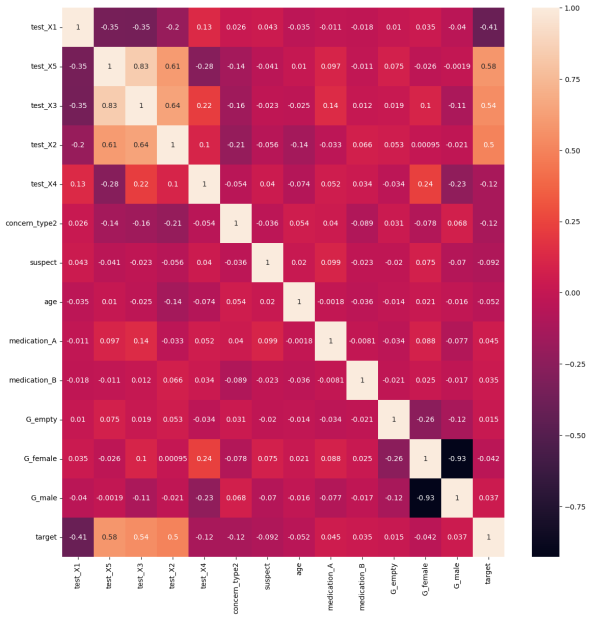
\includegraphics[width=0.5\linewidth]{Materials/feature_heatmap.png}
    \caption{Heat map of chosen features}
    \label{fig:heatmap}
\end{figure}


\subsection{Pipeline} 

For the steps in the in preprocessing who usage is not yet explained, several pipelines were constructed to test out various different methods and compare and contrast them they are as follow;

The essential steps included in every pipeline are:
Cleansing $\rightarrow$ Encoding $\rightarrow$ Feature selection $\rightarrow$ Train-test Split $\rightarrow$ \ldots $\rightarrow$ Balancing

Variations to this pipeline all occur within the ellipsis, they follow the order: Possible scaling $\rightarrow$ Possible outlier removal $\rightarrow$ Possible null imputation.

The methods employed for these are as follows;
Scaling: Min-max scaling
Null-Handling: Removal, Median imputation, Knn imputation
Outlier detection: DB-scan, Local outlier factor, Isolation forest

Initially a pipeline class was constructed to parse these, however the particulars of the functions meant it was more reasonable to call the functions directly. 

Some combinations were avoided, in particular if DB-scan, Local-outlier-factor or Knn were used then scaling is considered a requirement, whilst it is possible these algorithms can work without scaling they all use distance metrics and as such if data isn't scaled it is likely to preference features unnecessarily.

Due to time limitations of all possible combinations only a selection were tried. The particular pipelines attempted are discussed in results and evaluation of section \ref{learning}

\section{Supervised learning}\label{learning}

First examined are supervised learning techniques, I.e. learning techniques where the data is labeled with the target variable.

\subsection{Model choices}

Three models were tried for each pipeline used, those being k-nearest neighbour, random-forest and support vector regression. 

The initial parameters of these algorithms were set as the default given the default settings are reasonably good for classification problems they were as follows;
\begin{itemize}
    \item \textbf{Knn:} 7 nearest neighbours
    \item \textbf{SVC:} Kernel was radial bias function (rbf), and a margin of 1 (C)
    \item \textbf{Random forest:} 100 estimators, no max depth, minimum samples per split of 2 and a random state of 404 for reproducibility
\end{itemize}

\subsection{Results}

The results are given by algorithm by pipeline, with each score being given to 3 significant figures. The last test used a combination approach to outlier detection by combining Local outlier factor and DB-scan to search for outliers only agreed upon by both, in other words points that are both in sparse regions and not well clustered.

\begin{table}[H]
    \centering
    \begin{tabular}{|c|c|c|c|}
    \hline
         Model & F1 Score  & Precision  & Accuracy  \\
    \hline
        K-nearest Neighbours & 0.674 & 0.620 & 0.839 \\
    \hline
        Support Vector Classification & 0.801 & 0.777 & 0.925 \\
    \hline
        Random Forest & 0.939 & 0.904 & 0.979 \\
    \hline
    \end{tabular}
    \caption{Only Null Removal}
    \label{tab:my_label}
\end{table}

%Template pipeline with median imputation: 

\begin{table}[h]
    \centering
    \begin{tabular}{|c|c|c|c|}
    \hline
    Model & F1 Score  & Precision  & Accuracy  \\
    \hline
    K-nearest Neighbours &  0.708 & 0.667 & 0.856 \\
    \hline
    Support Vector Classification & 0.818 & 0.809 & 0.926 \\
    \hline
    Random Forest & 0.956 & 0.935 & 0.983 \\
    \hline
    \end{tabular}
    \caption{Only Median Imputation}
    \label{tab:my_label}
\end{table}

%Template pipeline with scaling and null removal:

\begin{table}[H]
    \centering
    \begin{tabular}{|c|c|c|c|}
    \hline
    Model & F1 Score & Precision & Accuracy  \\
    \hline
    K-nearest Neighbours & 0.625 & 0.592 & 0.729 \\
    \hline
    Support Vector Classification & 0.621 & 0.570 & 0.761 \\
    \hline
    Random Forest & 0.921 & 0.875 & 0.972 \\
    \hline
    \end{tabular}
    \caption{Scaling and Null removal}
    \label{tab:my_label}
\end{table}

% Template pipeline with scaling and median imputation

\begin{table}[H]
    \centering
    \begin{tabular}{|c|c|c|c|}
    \hline
    Model & F1 Score  & Precision  & Accuracy  \\
    \hline
    K-nearest Neighbours & 0.640 & 0.593 & 0.755 \\
    \hline
    Support Vector Classification & 0.663 & 0.599 & 0.794 \\
    \hline
    Random Forest & 0.933 & 0.888 & 0.979 \\
    \hline
    \end{tabular}
    \caption{Scaling and median imputation}
    \label{tab:my_label}
\end{table}

% Template pipeline with scaling and Knn imputation:

\begin{table}[H]
    \centering
    \begin{tabular}{|c|c|c|c|}
    \hline
      Model & F1 Score & Precision & Accuracy \\
    \hline
         K-nearest Neighbours & 0.639 & 0.592 & 0.762 \\
    \hline
        Support Vector Classification & 0.670 & 0.607 &0.793 \\
    \hline
         Random Forest & 0.922 & 0.878 & 0.973 \\
    \hline
    \end{tabular}
    \caption{Scaling and knn imputation}
    \label{tab:my_label}
\end{table}

% Template pipeline with, scaling, DB-scan and Knn imputation:

\begin{table}[H]
    \centering
    \begin{tabular}{|c|c|c|c|}
    \hline
         Model & F1 Score  & Precision  & Accuracy  \\
    \hline
         K-nearest Neighbours & 0.625 & 0.592 & 0.729 \\
    \hline
    Support Vector Classification & 0.621 & 0.570 & 0.761 \\
    \hline
         Random Forest & 0.921 & 0.875 & 0.972 \\
    \hline
    \end{tabular}
    \caption{Scaling, DB-scan and Knn imputation}
    \label{tab:my_label}
\end{table}

%Template with, scaling, Local outlier factor and Knn imputation:

\begin{table}[H]
    \centering
    \begin{tabular}{|c|c|c|c|}
    \hline
         Model & F1 Score & Precision & Accuracy \\
    \hline
         K-nearest Neighbours & 0.661 & 0.611 & 0.779 \\
    \hline
         Support Vector Classification & 0.683 & 0.623 & 0.814 \\
    \hline
         Random Forest & 0.919 & 0.872 & 0.971 \\
    \hline
    \end{tabular}
    \caption{Scaling, Local outlier factor and Knn imputation}
    \label{tab:my_label}
\end{table}

%Template with, scaling, Isolation forest and Knn imputation:

\begin{table}[H]
    \centering
    \begin{tabular}{|c|c|c|c|}
    \hline
         Model & F1 Score  & Precision  & Accuracy  \\
    \hline
         K-nearest Neighbours & 0.652 & 0.610 & 0.769 \\
    \hline
         Support Vector Classification & 0.664 & 0.606 & 0.789 \\
    \hline
         Random Forest & 0.944 & 0.912 & 0.980 \\
    \hline
    \end{tabular}
    \caption{Scaling, Isolation forest and Knn imputation}
    \label{tab:my_label}
\end{table}

%template with, scaling, BD-Scan, LOcal outlier factor and Knn imputation

\begin{table}[H]
    \centering
    \begin{tabular}{|c|c|c|c|}
    \hline
         Model & F1 Score & Precision & Accuracy \\
    \hline
         K-nearest Neighbours & 0.636 & 0.589 & 0.756 \\
    \hline
         Support Vector Classification & 0.688 & 0.629 & 0.806 \\
    \hline
         Random Forest & 0.922 & 0.878 & 0.973 \\
    \hline
    \end{tabular}
    \caption{Scaling, Combination of DB-Scan and Local outlier factor and Knn imputation}
    \label{tab:my_label}
\end{table}


\subsection{Interpretation}

As can be seen in the results tables, Random forest massively outperforms both K-nearest neighbours and Support vector classification. The implication of this is that the parameters for SVC and KNN could do with being tuned. To test this the best performing model (aside Only median imputation, since scaling should improve Knn) is used with a grid search to explore the parameter space for all the algorithms. The model in question is Scaling, Local outlier Factor and Knn imputation. 

Before examining the results from this to visualise the difference between the most accurate pipeline and least accurate, confusion matrices for all three models for each pipeline. From the results and the confusion matrices the general impression is the data is very highly correlated with the target variable. This is  backed up by implication in feature selection.

\begin{figure}
    \centering
    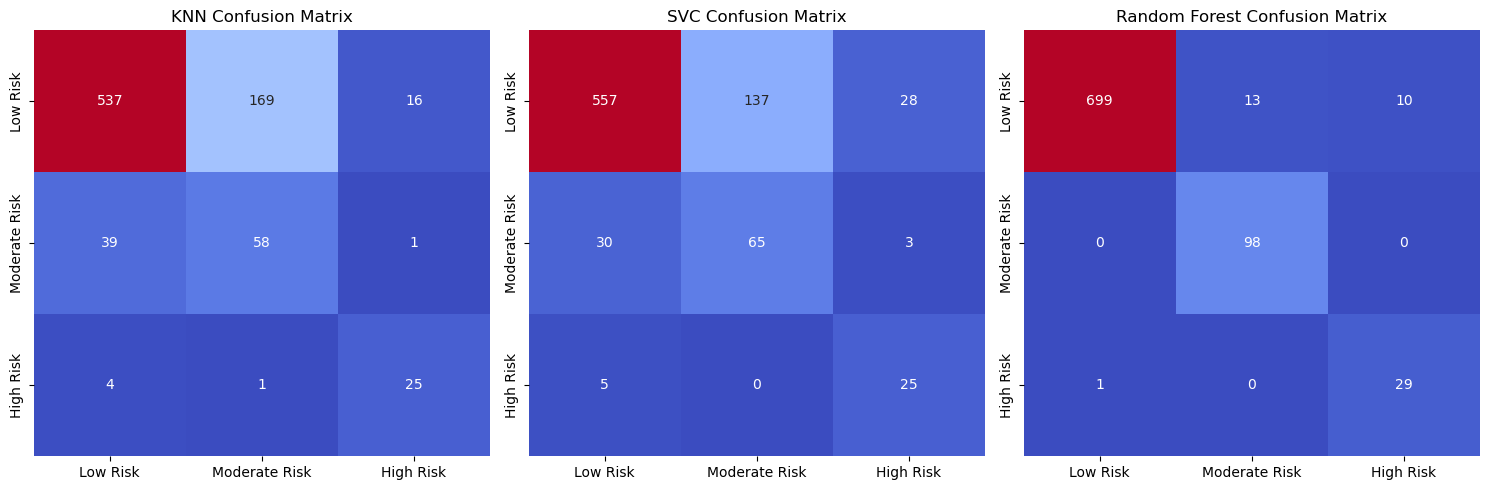
\includegraphics[width=0.5\linewidth]{DB KNN matrices.png}
    \caption{Confusion matrices of worst performing models}
    \label{fig:enter-label}
\end{figure}

\begin{figure}
    \centering
    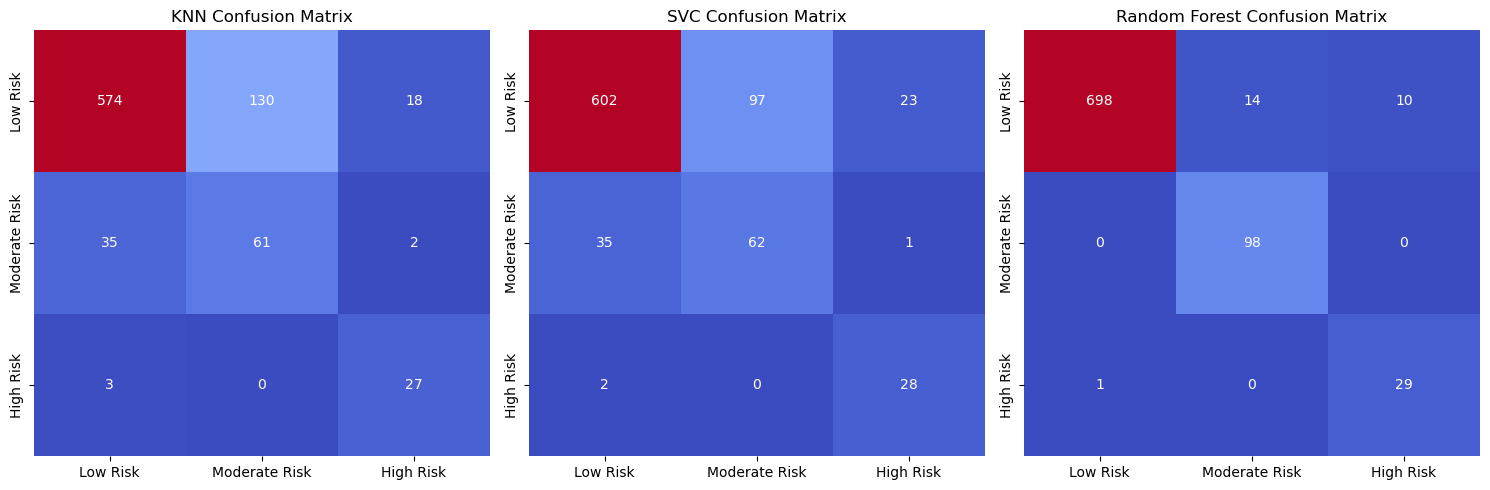
\includegraphics[width=0.5\linewidth]{LOF KNN matrices.png}
    \caption{Confusion matrices of best performing models}
    \label{fig:enter-label}
\end{figure}

The results of the grid-search didn't created better result for Support Vector Classification than initially found but no results better than the initial random forest values were found. 

The Random forest model was saved out, and then from it information was gathered. One such piece of information was feature importance seen in table \ref{tab:feat importance}. THis roughly corresponds to the results from the feature selection statistical tests.

\begin{table}[H]
    \centering
    \begin{tabular}{|c|c|c|c|}
    \hline
        Feature & Importance & Feature & Importance \\
    \hline
        test 1  &  0.374911 & medication A & 0.009889\\
    \hline
        test 2  &  0.215178 & G\_empty  &  0.003241 \\
    \hline
        test 5  &  0.192037 & G\_female  &  0.002349 \\
    \hline
        test 3  &  0.125815 & suspect  &  0.001982 \\
    \hline
        test 4   & 0.033378 & G\_male   & 0.001939 \\
    \hline
        concern type 2 &   0.023927 &   medication B  &  0.000937 \\
    \hline
        age  &  0.014418 &  & \\
    \hline
    \end{tabular}
    \caption{Feature importance in best model}
    \label{tab:feat importance}
\end{table}


\section{Unsupervised learning}

Unsupervised learning was briefly tried with the data set, K-means was the algorithm used. The elbow method was used to get an estimated of K. And it was found that K of 4 was the optimal number of clusters, which is somewhat surprising considering the high dimensionality of the data.

\begin{figure}[t]
    \centering
    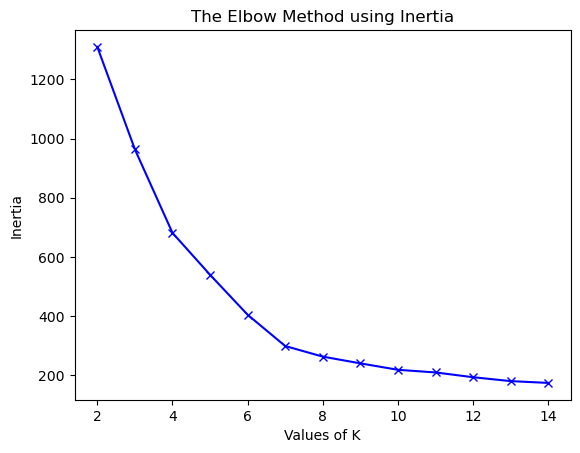
\includegraphics[width=0.5\linewidth]{Elbw method K means.png}
    \caption{Elbow method for K-Means}
    \label{fig:enter-label}
\end{figure}
\section{Summary/Conclusion}

In summary, this project has explored and examine a medical dataset thoroughly, proposed a number of preprocessing pipelines and compared them. Trained an ideal model to predict risk. Custom metrics over diagnosis rate and under diagnosis rate have been used to create novel models (resources saving vs cautious). 

Both supervised and unsupervised learning have been examined, various techniques have been explore some of them implemented and visualisations have been used to accompany much of the explanation.

\bibliographystyle{plainnat}
\bibliography{report_example}

\end{document}
